\documentclass[a4paper]{article}
\usepackage{fontspec}
\usepackage{hyperref}
\hypersetup{hidelinks,
	colorlinks=true,
	allcolors=black,
	pdfstartview=Fit,
	breaklinks=true
}
\usepackage{amsmath}
\usepackage{xpatch}

\ExplSyntaxOn
\xpatchcmd \fontspec_new_script:nn
  { \__fontspec_warning:nxx }
  { \__fontspec_info:nxx }
  {}{\fail}

\newfontscript{CJK}{hani}
\ExplSyntaxOff

\usepackage{xeCJK}
\usepackage{ctex}
\usepackage{lipsum}
\usepackage{graphicx}
\usepackage{geometry}
\usepackage{indentfirst}
\setlength{\parindent}{2em}
\setlength{\parskip}{1em}
% for check box
\usepackage{enumitem,amssymb}
% for check symbol 
\usepackage{pifont}
\usepackage{enumitem}
\usepackage{float}
\usepackage{listings}
\usepackage{color}


\definecolor{dkgreen}{rgb}{0,0.6,0}
\definecolor{gray}{rgb}{0.5,0.5,0.5}
\definecolor{mauve}{rgb}{0.58,0,0.82}

\lstset{frame=tb,
  language=Java,
  aboveskip=3mm,
  belowskip=3mm,
  showstringspaces=false,
  columns=flexible,
  basicstyle={\small\ttfamily},
  numbers=none,
  numberstyle=\tiny\color{gray},
  keywordstyle=\color{blue},
  commentstyle=\color{dkgreen},
  stringstyle=\color{mauve},
  breaklines=true,
  breakatwhitespace=true,
  tabsize=3
}

\newcommand{\cmark}{\ding{51}}% check mark
\newcommand{\done}{\rlap{$\square$}{\raisebox{2pt}{\large\hspace{1pt}\cmark}}\hspace{-2.5pt}}
\pagestyle{plain}

\begin{document}
\thispagestyle{empty}
\noindent\parbox[c]{.6\linewidth}{
	\linespread{1.3}
	\itshape  \par
    \  \par
    \  \par
    作品类别:\done 软件设计\ \ {\rlap{$\square$}{\large\hspace{1pt}}}\ \ 硬件制作\ \ {\rlap{$\square$}{\large\hspace{1pt}}}\ \ 工程实践 \par
}%



\begin{center}

\par\vspace{.2\textheight}

{\Large\textbf{密码学单人作品}\par}
\Large
\rule{\textwidth}{0.5mm}
\par\vspace{.05\textheight}
\Large{题目:混沌置乱的循环阶分析}

\medbreak
\par\vspace{.25\textheight}
\medbreak
黄柏熙 \quad PB23071429
\medbreak



\end{center}
\vfill
% 项目信息
\begin{center}
        \begin{tabular}{ | p{.95\hsize} | }
    \hline
    基本信息表 \\
    \hline
    作品题目:示例题目\\
    \hline
    作品类别:\done 软件设计\ \ {\rlap{$\square$}{\large\hspace{1pt}}}\ \ 硬件制作\ \ \ {\rlap{$\square$}{\large\hspace{1pt}}}\ \ 工程实践 \\
    \hline
    作品内容摘要:\\
    \par 量化评估Logistic、Cubic和Sine混沌映射构造置乱的循环特性:循环圈长度、每种长度的循环圈个数和总的循环阶,使用的方法为统计计算平均阶-N曲线\\
    \hline
关键词:\\
混沌置乱、循环阶、Logistic映射、Cubic映射、Sine映射
\\
\hline
\end{tabular}
\end{center}

\clearpage
\tableofcontents
\clearpage
\section{作品概述}
\subsection{引言}
网络已经成为人们沟通交流的主要平台,但是网络为我们的沟通交流提供了极大的便捷的同时,也存在许多信息安全的相关问题,特别是信息的传递,对信息加密
可以在一定的程度上保护信息的隐秘性,因此信息的加密是一项很值得研究的课题,本文评估了三种混沌映射:Logistic映射、Cubic映射和Sine映射的
置乱效果\par

\subsection{研究背景与意义}
随着数据化时代的到来,数据泄露、恶意攻击的问题日益突出,信息安全的重要性在不断增长。\par
1975年,美国数学家约克和美籍华人李天岩发表了《周期3意味着混沌》的文章,首次提出了“混沌”—词,阐述了混沌的数学定义,对混沌学的发展具有重大意义。自此以后,混沌研究开始蓬勃发展。\par
混沌是指在确定性动力学系统中,由于对初值敏感而表现出的类似随机的、不可预测的运动。混沌是确定的非线性系统中出现的内在随机性现象,其变化并非随机确貌似随机。\cite{ref1}\par
混沌映射被用于生成混沌序列,这是一种由简单的确定性系统产生的随机性序列。一般混沌序列具有以下主要特征:
\begin{enumerate}
  \item 随机性
  \item 非线性
  \item 对初值敏感依赖
  \item 遍历性
  \item 长期不可预测性
\end{enumerate}
等等,混沌映射有时也可以当作随机数生成器。本文利用混沌映射进行置乱,可以在图像、视频、通讯等领域应用,以保护隐私数据

\clearpage
\section{设计实现与方案}

\subsection{实验原理}
利用混沌映射的随机性,将获得的N个数进行排序后,这N个数的下标也呈现随机性,再进行一步变换后达到置乱的效果。\par
循环圈长度越长,需要进行的置乱越多,更难回复原始数据,安全性更强;循环圈个数越多,可能意味着局部性越强(短循环越多),
安全性可能下降;总循环长度越高,安全性越强,因为总循环长度反映的是最少需要多少次置乱才能恢复成初始状态。

\subsection{构造置乱算法}
\begin{enumerate}
  \item 选定一个混沌映射
  \item 选定参数$\mu$和初始值(即种子)$x_0$,迭代M轮得到$x_M$,继续迭代计算$x_{M+1}\sim x_{M+N}$
  \item 将这N个数按照大小排序,以每个数的位置为置乱索引。例如,$x_i$被排在第j,位,则置乱中将第i个数移至第j位
\end{enumerate}
选用一些数据进行小范围的循环圈长度、循环圈个数以及总循环长度(阶)测试,然后固定N进行随机的混沌因数和种子计算N的平均阶,绘制“平均阶-N”的曲线分析

\subsection{选择混沌映射}
本文选择了三种混沌映射:\par
Logistic映射:
$$
x_{n+1} = \mu x_n(1-x_n) \quad (0<x<1)
$$
在$3.57<\mu<4$呈现混沌特性\par
Cubic映射:
$$
x_{n+1} = rx_n(1-x_n^2) \quad (0<x<1)
$$
在$2.5<r<3$呈现混沌特性\par
Sine映射:
$$
x_{n+1} = \frac{4}{a}\sin(\pi x_n) \quad (-1<x<1)
$$
在$0<a<4$呈现混沌特性\par
\clearpage
\section{系统测试与结果}

\subsection{测试方案}
选择在python平台上进行代码编写,对于循环圈长度、循环圈个数和阶采用几组随机数据测评;对于“平均阶-N”采用生成随机
的$x_0$和$\mu$,并生成数据,将数据写入Excel表格内,再利用Origin分析软件进行拟合的方式进行分析。

\subsection{功能测试与分析}
\subsubsection{Logistic}
由于$3.57<\mu<4 \quad (0<x<1)$中呈现混沌特性,我选取以下几组数据[($x_0,\mu,N$)](M选择1000)进行测试:
\begin{lstlisting}
  (0.66,3.66,40)                (0.66,3.66,80)                 (0.66,3.66,120)
  循环数量 4                    循环数量 6                     循环数量 6
  循环长度 [33,3,3,1]           循环长度 [27,19,27,3,2,2]      循环长度 [48,48,7,7,3,7]
  阶 33                         阶 1026                        阶 336
  循环 33 有 1 个               循环 27 有 2 个                循环 48 有 2 个
  循环 3 有 2 个                循环 19 有 1 个                循环 7 有 3 个
  循环 1 有 1 个                循环 3 有 1 个                 循环 3 有 1 个
                                循环 2 有 2 个
\end{lstlisting}
可以看到,最大循环长度基本是随N递增而增大的,由于第三组中最大的循环长度相等,所以阶会比第二组小。对于N比较小的
情况下,Logistic混沌置乱下的小循环比较多,这个对于安全性是不是很有利。\par
\newpage
以下是经过拟合的“平均阶-N”图像:
\begin{figure}[H]
  \centering
  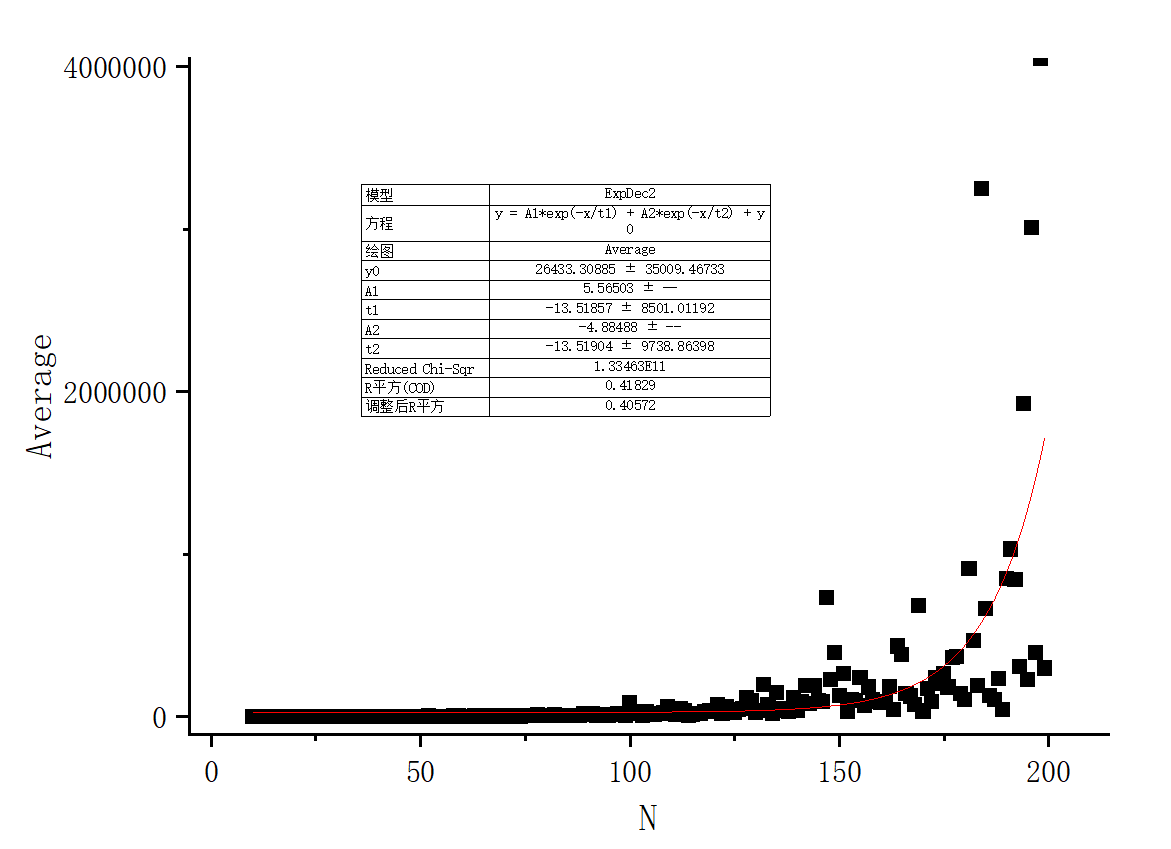
\includegraphics[width=0.8\textwidth]{imgs/logistic.png}
  \caption{Logistic映射置乱}
  \label{Logistic}
\end{figure}
可以看到,平均阶-N图像基本是以指数增长的形式增长的,也就是说,N越大,复原置乱所需要的置乱次数基本成指数级增长,
在N为200左右的时候,平均阶的数量级在$10^5\sim 10^6$,在N足够大的是后表现良好
\subsubsection{Cubic}
Cubic映射在$2.5<3r \quad (0<x<1)$的时候呈现混沌特性,选取以下几组数据进行测试:
\begin{lstlisting}
  (0.68,2.83,40)                (0.68,2.83,80)                (0.68,2.83,120)
  循环数量 2                    循环数量 6                    循环数量 6
  循环长度 [37,3]               循环长度 [39,16,4,16,4,1]     循环长度 [61,27,27,2,2,1]
  阶 111                        阶 624                        阶 3294
  循环 37 有 1 个               循环 39 有 1 个               循环 61 有 1 个
  循环 3 有 1 个                循环 16 有 2 个               循环 27 有 2 个
                                循环 4 有 2 个                循环 2 有 2 个
                                循环 1 有 1 个                循环 1 有 1 个
\end{lstlisting}
可以看出测试数据中阶关于N的增长比较大,性能相较于上面讨论的Logistic混沌置乱更强,以下是经过拟合的“平均阶-N”图像:

\begin{figure}[H]
  \centering
  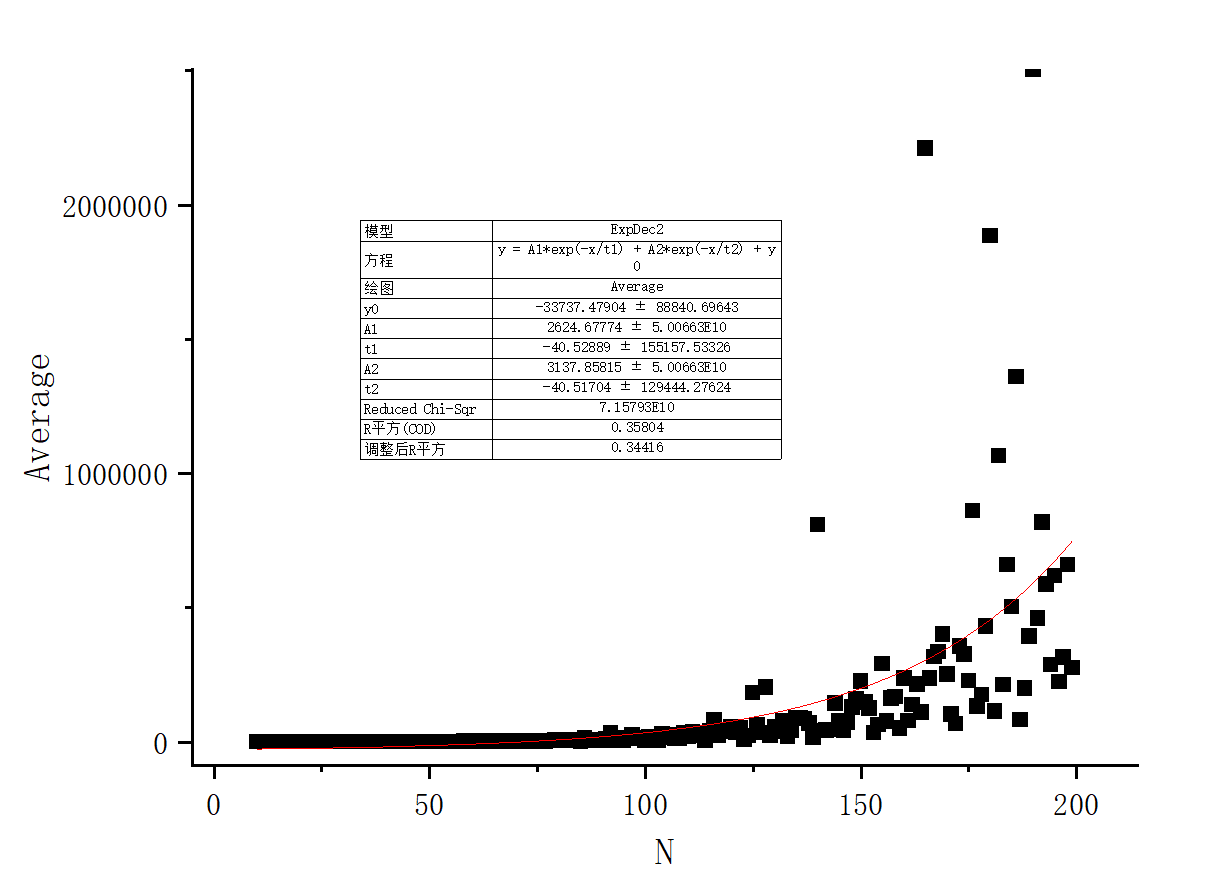
\includegraphics[width=0.8\textwidth]{imgs/cubic.png}
  \caption{Cubic映射置乱}
  \label{Cubic}
\end{figure}

从曲线整体的走势可以看出Cubic混沌置乱在N相对较小的情况下,可以带来相较于Logistic混沌置乱更强的安全性,
复原一个序列需要的计算量更大。

\subsubsection{Sine}
\begin{lstlisting}
  (0.31,3.62,40)                    (0.31,3.62,80)            (0.31,3.62,120)
  循环数量 8                        循环数量 4                循环数量 10
  循环长度 [10,2,7,2,7,10,1,1]   循环长度 [25,33,11,11]       循环长度 [13,65,2,3,5,7,13,7,3,2]
  阶 70                             阶 825                    阶 2730
  循环 10 有 2 个                   循环 25 有 1 个           循环 13 有 2 个
  循环 2 有 2 个                    循环 33 有 1 个           循环 65 有 1 个
  循环 7 有 2 个                    循环 11 有 2 个           循环 2 有 2 个
  循环 1 有 2 个                                              循环 3 有 2 个
                                                              循环 5 有 1 个
                                                              循环 7 有 2 个
\end{lstlisting}

根据测试数据,Sine映射的循环圈数量较多,影响局部安全性。

\begin{figure}[H]
  \centering
  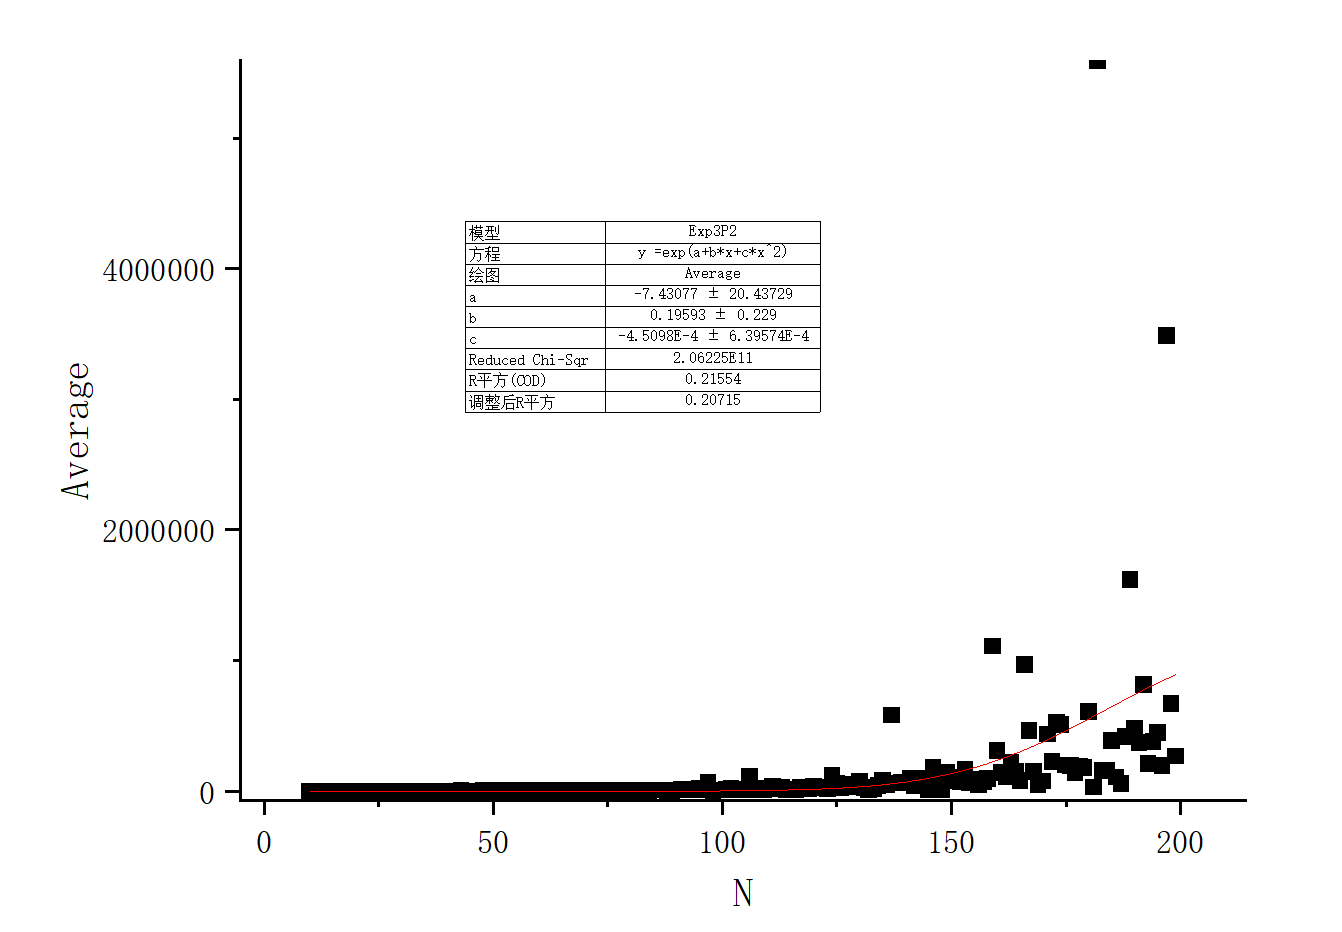
\includegraphics[width=0.8\textwidth]{imgs/sine.png}
  \caption{Sine映射置乱}
  \label{Sine}
\end{figure}

从图像可以看出Sine混沌置乱的平均阶增长较为缓慢,相较于前面两个混沌映射,安全性更弱

\clearpage
\section{应用前景}

混沌置乱可以应用在图像的加密,加密效果如下图所示:\par
原图、Logistic加密、解密后的图像:
\begin{figure}[H]
  \centering
  
\includegraphics[width=0.8\textwidth]{imgs/lena.jpg}
  \caption{Lena图}
  \label{Lena}
\end{figure}

\begin{figure}[H]
  \centering
  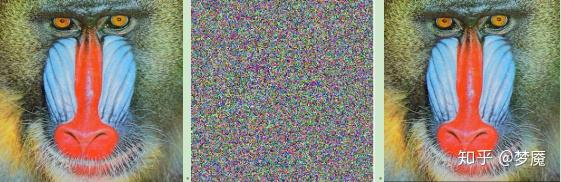
\includegraphics[width=0.8\textwidth]{imgs/baboom.jpg}
  \caption{Baboom图}
  \label{Baboom}
\end{figure}
图片来源:\cite{ref1}

由于计算复杂度低,混沌置乱适合实时加密,还可以用于视频流加密、通信安全等领域。

\clearpage
\section{结论}

本文对三个不同的混沌置乱进行了简短的分析,总结得出三个置乱中Cubic混沌置乱的效果最好,而且置乱的安全性
基本随着N的增大呈指数级增长,N足够大时可以获得较强的安全性。

\clearpage
\begin{thebibliography}{99}
    \bibitem{ref1} 知乎用户.基于混沌Logistic加密算法的图片加密与还原[EB/OL].知乎专栏, 2021.\url{https://zhuanlan.zhihu.com/p/183788811}
\end{thebibliography}

\end{document}